\chapter{Problemas para o 7º ano.}
%==============================================================================================
\section{Expressões Numéricas}
\begin{list}{\textbf{Questão \arabic{quest}.}}{\usecounter{quest}}
%define a margem da lista.	
%\setlength{\labelwidth}{-2mm} \setlength{\parsep}{0mm}
%\setlength{\topsep}{0mm} \setlength{\leftmargin}{-2mm}
\renewcommand{\labelenumi}{(\alph{enumi})}

\item Calcule o valor das expressões
	\begin{multicols}{2}
	\begin{enumerate}[a)]
	\item $25-[10+(7-4)] =    (R:12)$
	\item $32+[10-(9-4)+8] =                         (R:45)$
	\item $45-[12-4+(2+1)] =                          (R:34)$
	\item $70-\{20-[10-(5-1)]\} =                     (R:56)$
	\item $28+\{13-[6-(4+1)+2]-1\} =              (R:37)$
	\item $53-\{20-[30-(15-1+6)+2]\} =           (R:45)$
	\item $62-\{16-[7-(6-4)+1]\} =                   (R:52)$
	\item $20-\{8+[3+(8-5)-1]+6\} =                (R:1)$
	\item $15+\{25-[2-(8-6)]+2\} =                   (R:42)$
	\item $56-[3+(8-2)+(51-10)-(7-2)] =          (R:11)$
	\end{enumerate}
	\end{multicols}

\item Calcule as expressões
	\begin{multicols}{2}
	\begin{enumerate}[a)]
		\item $3\cdot75+3\cdot25= (R:300)$
		\item $5\cdot97+5\cdot3= (R:500 )$
		\item $4\cdot101+4\cdot99= (R:800)$
		\item $20\cdot47+80\cdot47= (R:4700)$
		\item $12+16:8\cdot3-5= (R:13)$
		\item $100-6\cdot7+8:2 = (R:62)$
		\item $64:8+5\cdot5-3= (R: 30)$
		\item $1+3+5\cdot7-9:3 = (R:36)$
	\end{enumerate}
	\end{multicols}

\item Calcule o valor das expressões:
	\begin{multicols}{2}
	\begin{enumerate}[a)]
		\item $7+15:3                    = (R:12)$
		\item $4\cdot5+1                     = (R:21)$
		\item $10:2+8                    = (R:13)$
		\item $32+12:2                  = (R:38)$
		\item $20:10+10                = (R:12)$
		\item $7\cdot3-2\cdot5                   = (R:11)$
		\item $40-2\cdot4+5                 = (R:37)$
		\item $4\cdot3+10:2                 = (R:17)$
		\item $50-16:8+7                 = (R:55)$
		\item $32:4:2:2                    = (R:2)$
	\end{enumerate}
	\end{multicols}

\item Calcule o valor das expressões
	\begin{multicols}{2}
	\begin{enumerate}[a)]
		\item $(13+2)\cdot3+5            = (R:50)$
		\item $(7+2\cdot(3-1)              = (R:18)$
		\item $(4+2\cdot5)-3                = (R:11)$
		\item $20-(15+6:3)                        = (R:3)$
		\item $15+[6+(8-4:2)]                    = (R:27)$
		\item $40-[3+(10-2):2]                    = (R:33)$
		\item $[30+2\cdot(5-3)]\cdot2-10              = (R:58)$
		\item $10+[4+(7\cdot3+1)]-3              = (R:33)$
	\end{enumerate}
	\end{multicols}


\item Calcule o valor das expressões
	\begin{multicols}{2}
	\begin{enumerate}[a)]
		\item $(3+2)\cdot(5-1)+4                    = (R:24)$
		\item $82-8\cdot7:(4-1\cdot3)                   = (R:26)$
		\item $25-[10-(2\cdot3+1)]                 = (R:22)$
		\item $70-[12+(5\cdot2-1)+6]             = (R:43)$
		\item $8:2+[15-(4\cdot2+1)]                = (R:10)$
		\item $9+[4+2\cdot(6-4)+(2+5)]-8                   = (R:16)$
		\item $50+\{10-2\cdot[(6+4:2)-(10-3)]\}                      = (R:58)$
		\item $180:\{10+2\cdot[20-45:(13-2\cdot5)]\}                    = (R:9)$
	\end{enumerate}
	\end{multicols}



\item Calcule o valor das expressões:
	\begin{multicols}{2}
	\begin{enumerate}[a)]
		\item $70:7-1                     = (R:9)$
		\item $20+3\cdot2= (R:26)$
		\item $30+10:10                = (R:31)$
		\item $150-7\cdot12                = (R:66)$
		\item $48:16+20:4             = (R:8)$
		\item $10-8:2+3                 = (R:9)$
		\item $30:5-1+2\cdot3             = (R:11)$
	\end{enumerate}
	\end{multicols}


\item Calcule as expressões:
	\begin{multicols}{2}
	\begin{enumerate}[a)]
		\item $(3+4)\cdot(9-8)                         = (R:7)$
		\item $(20+8):(3+4)                      = (R:4)$
		\item $15+8\cdot(2+3)                        = (R:55)$
		\item $(5+3\cdot2)-1                           = (R:10)$
		\item $25+(8:2+1)-1                      = (R:29)$
		\item $15+[5\cdot(8-6:2)]                    = (R:40)$
		\item $50-[13-(10-2):2]                 = (R:41)$
		\item $[40+2\cdot(7-5)]\cdot2-20             = (R:68)$
	\end{enumerate}
	\end{multicols}

\item Calcule o valor das expressões:
	\begin{multicols}{2}
	\begin{enumerate}[a)]
		\item $16+[10-(18:3+2)+5]                       = (R: 23)$
		\item $25-[12-(3\cdot2+1)]                             = (R: 20)$
		\item $90-[25+(5\cdot2-1)+3]                         = ( R: 53)$
		\item $45+[(8\cdot5-10:2)+(18:6-2)]              = (R: 81)$
		\item $50-2\cdot\{7+8:2-[9-3\cdot(5-4)]\}              = (R: 40)$
		\item $100-3\cdot\{5+8:2-[3\cdot(7-6)]\}               = (R: 82)$
	\end{enumerate}
	\end{multicols}


\item Determine o valor de cada expressão
	\begin{multicols}{2}
	\begin{enumerate}[a)]
		\item $1000 - [(2 \cdot 4 - 6) + ( 2 + 6 \cdot 4)]      = (R: 972)$
		\item $60 + 2 \cdot \{[ 4 \cdot ( 6 + 2 ) - 10 ] + 12\}      = ( R: 128 )$
		\item $[( 4 + 16 \cdot 2) \cdot 5 - 10] \cdot 100   = (R: 17.000)$
		\item $\{ 10 + [ 5 \cdot ( 4 + 2 \cdot 5) - 8] \cdot 2 \} - 100  = ( R: 34)$
		\item $80 - 5 \cdot ( 28 - 6 \cdot 4 ) + 6 - 3 \cdot 4      = (R: 54)$
	\end{enumerate}
	\end{multicols}


\item Calcule
	\begin{multicols}{2}
	\begin{enumerate}[a)]
		\item $4 \cdot ( 10 + 20 + 15 + 30)  = (R: 300)$
		\item $(10 \cdot 6 + 12 \cdot 4 + 5 \cdot 8 ) - 40   = (R: 108)$
		\item $[ 6 \cdot ( 3 \cdot 4 - 2 \cdot 5) - 4 ] + 3 \cdot ( 4 - 2) - ( 10 : 2 ) = (R: 9)$
		\item $67 + \{ 50 \cdot [ 70 : ( 27 + 8 ) + 18 : 2 ] + 21 \}  = (R:638)$
		\item $[ 30 \cdot ( 9 - 6)] + [ 30 : ( 9 + 6 ) ]  = (R: 92)$
		\item $58 - [ 20 - ( 3 \cdot 4 - 2) : 5 ]= (R: 40)$
		\item $40 + 2 \cdot [ 20 - ( 6 + 4 \cdot 7 ) : 2 ] = ( R: 46)$
	\end{enumerate}
	\end{multicols}
\end{list}

%==============================================================================================
%=============================================================================================
\section{Geometria Espacial}

\begin{list}{\textbf{Questão \arabic{quest}.}}{\usecounter{quest}}
%define a margem da lista.	
%\setlength{\labelwidth}{-2mm} \setlength{\parsep}{0mm}
%\setlength{\topsep}{0mm} \setlength{\leftmargin}{-2mm}
\renewcommand{\labelenumi}{(\alph{enumi})}

\item  Observe a caixa representada abaixo:
\begin{center}
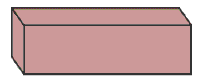
\includegraphics[scale=1]{figuras/fig80.png}
\end{center}
Uma planificação dessa caixa é:
\begin{multicols}{4}
\begin{enumerate}[a)]
	\item 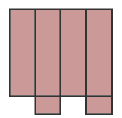
\includegraphics[scale=0.7]{figuras/fig80_a.png}
	\item 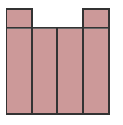
\includegraphics[scale=0.7]{figuras/fig80_b.png}
	\item 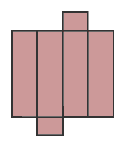
\includegraphics[scale=0.7]{figuras/fig80_c.png}
	\item 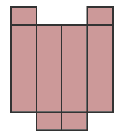
\includegraphics[scale=0.7]{figuras/fig80_d.png} 
\end{enumerate}
\end{multicols}

\item A forma geométrica espacial que pode ser associada à planificação abaixo é:
\begin{multicols}{2}
	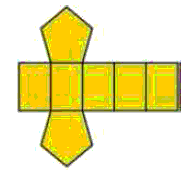
\includegraphics[scale=0.7]{figuras/fig81.png}
	\begin{enumerate}[a)]
		\item um cilindro
		\item uma pirâmide de base pentagonal 
		\item um prisma de base pentagonal.
		\item um paralelepípedo	
	\end{enumerate}
\end{multicols}

\item As figuras 1, 2 e 3 correspondem, respectivamente, às planificações dos sólidos:
\begin{center}
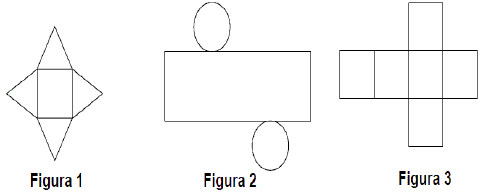
\includegraphics[scale=0.6]{figuras/fig82.png}
\end{center}
\begin{multicols}{4}
\begin{enumerate}[a)]
	\item Cubo, cone, pirâmide.
	\item Pirâmide, cilindro, cubo.
	\item Cubo, cilindro, pirâmide.
	\item Pirâmide, cone, cubo.
\end{enumerate}
\end{multicols}
\item Analise estes desenhos de poliedros e determine em cada um deles o número de vértices(V), o número de faces (F) e o número de arestas (A).
\begin{center}
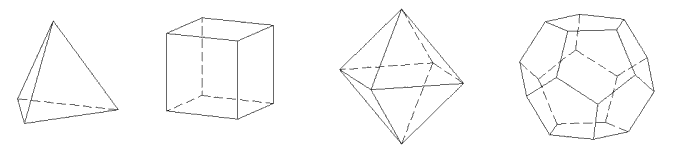
\includegraphics[scale=0.9]{figuras/fig83.png}
\end{center}

\end{list}

%==============================================================================================
%=============================================================================================
\section{Geometria Plana}

\begin{list}{\textbf{Questão \arabic{quest}.}}{\usecounter{quest}}
%define a margem da lista.	
%\setlength{\labelwidth}{-2mm} \setlength{\parsep}{0mm}
%\setlength{\topsep}{0mm} \setlength{\leftmargin}{-2mm}
\renewcommand{\labelenumi}{(\alph{enumi})}

\item Desenhe um polígono convexo e outro não convexo.
\item Calcule o número de diagonais em:
\begin{multicols}{2}
\begin{enumerate}[a)]
\item um polígono convexo de 11 lados;
\item um decágono(dez lados) convexo;
\item um icoságono(vinte lados) convexo;
\item um polígono convexo de 13 lados.
\end{enumerate}
\end{multicols}

\end{list}

%==============================================================================================
%=============================================================================================
\section{Números racionais}
\subsection{Atividades Introdutórias}
\begin{list}{\textbf{Questão \arabic{quest}.}}{\usecounter{quest}}
%define a margem da lista.	
%\setlength{\labelwidth}{-2mm} \setlength{\parsep}{0mm}
%\setlength{\topsep}{0mm} \setlength{\leftmargin}{-2mm}
\renewcommand{\labelenumi}{(\alph{enumi})}


\item Simplifique as frações.
\begin{multicols}{6}
\begin{enumerate}[a)]
	\item $\dfrac{10}{20}$
	\item $\dfrac{15}{35}$
	\item $\dfrac{6}{2}$
	\item $\dfrac{50}{60}$
	\item $\dfrac{20}{100}$
	\item $\dfrac{35}{40}$
	\item $\dfrac{16}{24}$
	\item $\dfrac{12}{16}$
	\item $\dfrac{20}{90}$
	\item $\dfrac{49}{63}$
	\item $\dfrac{12}{21}$
	\item $\dfrac{13}{15}$
	\item $\dfrac{19}{25}$
	\item $\dfrac{45}{82}$
	\item $\dfrac{50}{10}$
	\item $\dfrac{54}{27}$
	\item $\dfrac{9}{72}$
	\item $\dfrac{6}{17}$
	\item $\dfrac{65}{70}$
	\item $\dfrac{2}{3}$
	\item $\dfrac{7}{42}$
	\item $\dfrac{11}{120}$
	\item $\dfrac{56}{64}$
	\item $\dfrac{85}{24}$			
\end{enumerate}
\end{multicols}

\item Para cada item, escreva duas frações equivalentes.
\begin{multicols}{6}
\begin{enumerate}[a)]
	\item $\dfrac{1}{2}$		
	\item $\dfrac{2}{5}$		
	\item $\dfrac{7}{2}$		
	\item $\dfrac{8}{9}$		
	\item $\dfrac{5}{7}$		
	\item $\dfrac{9}{13}$		
	
	\item $\dfrac{2}{7}$		
	\item $\dfrac{11}{2}$		
	\item $\dfrac{7}{10}$		
	\item $\dfrac{9}{17}$		
	\item $\dfrac{1}{9}$		
	\item $\dfrac{8}{5}$		

	\item $\dfrac{10}{11}$		
	\item $\dfrac{7}{4}$		
	\item $\dfrac{4}{7}$		
	\item $\dfrac{2}{3}$		
	\item $\dfrac{6}{2}$		
	\item $\dfrac{20}{21}$		

	\item $\dfrac{21}{35}$		
	\item $\dfrac{1}{100}$		
	\item $\dfrac{1}{1000}$		
	\item $\dfrac{4}{50}$		
	\item $\dfrac{9}{40}$		
	\item $\dfrac{10}{100}$		
\end{enumerate}
\end{multicols}

\item Calcule:
\begin{multicols}{4}
\begin{enumerate}[a)]
	\item $mmc(2,4)=$
	\item $mmc(4,5)=$
	\item $mmc(6,7)=$
	\item $mmc(3,4)=$
	\item $mmc(8,12)=$

	\item $mmc(6 ,4 )=$
	\item $mmc(4,6)=$
	\item $mmc(10,100 )=$
	\item $mmc(6,18)=$
	\item $mmc(12,24)=$

	\item $mmc(13,9)=$
	\item $mmc(6,7)=$
	\item $mmc(9,10)=$
	\item $mmc(3,5)=$
	\item $mmc(6,11)=$

	\item $mmc(2,3,5)=$
	\item $mmc(3,4,5)=$
	\item $mmc(3,6,12)=$
	\item $mmc(5,10,20)=$
	\item $mmc(3,4,17)=$

\end{enumerate}
\end{multicols}

\item Reduza ao menor denominador comum as seguintes frações:
\begin{multicols}{3}
\begin{enumerate}[a)]
	\item $\dfrac{9}{4}\ , \dfrac{6}{7}$
	\item $\dfrac{7}{9}\ ,\ \dfrac{5}{3}$
	\item $\dfrac{3}{10}\ ,\ \dfrac{7}{15}$

	\item $\dfrac{1}{8}\ ,\ \dfrac{1}{5},\ \dfrac{1}{10}$
	\item $\dfrac{3}{4}\ ,\ \dfrac{7}{6},\ \dfrac{8}{9}$
	\item $\dfrac{5}{12}\ ,\ \dfrac{3}{8},\ \dfrac{1}{6}$
\end{enumerate}
\end{multicols}

\item Escreva em forma de fração imprópria:
\begin{multicols}{6}
\begin{enumerate}[a)]
	\item $4\frac{1}{2}$
	\item $7\frac{2}{3}$
	\item $5\frac{3}{4}$
	\item $1\frac{4}{7}$
	\item $10\frac{1}{2}$
	\item $11\frac{1}{5}$
\end{enumerate}
\end{multicols}

\item Escreva em forma de mista as seguintes frações impróprias:
\begin{multicols}{6}
\begin{enumerate}[a)]
	\item $\dfrac{16}{5}$
	\item $\dfrac{17}{3}$
	\item $\dfrac{31}{3}$
	\item $\dfrac{9}{2}$
	\item $\dfrac{11}{7}$
	\item $\dfrac{20}{6}$
\end{enumerate}
\end{multicols}

\item Calcule:
\begin{multicols}{3}
\begin{enumerate}[a)]
	\item $2\frac{1}{5} + \dfrac{3}{4}$
	\item $1\frac{1}{6} + 1\frac{1}{9}$
	\item $\dfrac{7}{10} + 2\frac{3}{4}$
\end{enumerate}
\end{multicols}

\item Calcule e simplifique, quando for possível, o resultado:
\begin{multicols}{3}
\begin{enumerate}[a)]
	\item $\dfrac{5}{7} - \dfrac{2}{7} = $
	\item $\dfrac{7}{8} - \dfrac{3}{8} = $
	\item $\dfrac{2}{9} - \dfrac{2}{9} = $

	\item $\dfrac{6}{6} - \dfrac{1}{6} = $
	\item $\dfrac{9}{10} - \dfrac{1}{10} = $
	\item $\dfrac{7}{12} - \dfrac{5}{12} = $

	\item $\dfrac{7}{5} - \dfrac{3}{5} + \dfrac{2}{5} = $
	\item $\dfrac{7}{9} + \dfrac{3}{9} - \dfrac{4}{9} = $
	\item $\dfrac{8}{8} - \dfrac{7}{8} + \dfrac{1}{8} = $
\end{enumerate}
\end{multicols}

\item Qual alternativa representa a fração 9/2 em números decimais?
\begin{multicols}{4}
\begin{enumerate}[a)]
	\item 3,333
	\item 4,25
	\item 5,01
	\item 4,5
\end{enumerate}
\end{multicols}

\item Qual alternativa representa a fração 35/1000 em números decimais?
\begin{multicols}{4}
\begin{enumerate}[a)]
	\item 0,35
	\item 3,5
	\item 0,035
	\item 35
\end{enumerate}
\end{multicols}

\item Qual é a alternativa que representa o número 0,65 na forma de fração?
\begin{multicols}{4}
\begin{enumerate}[a)]
	\item $\displaystyle\frac{65}{10}$
	\item $\displaystyle\frac{65}{100}$
	\item $\displaystyle\frac{65}{1000}$
	\item $\displaystyle\frac{65}{10000}$
\end{enumerate}
\end{multicols}

\item Observe as frações e suas respectivas representações decimais.
\begin{multicols}{4}
\begin{enumerate}[a)]
	\item $\displaystyle\frac{3}{1000}=0,003$
	\item $\displaystyle\frac{2367}{100}=23,67$
	\item $\displaystyle\frac{129}{1000}-0,129$
	\item $\displaystyle\frac{65}{10000}=0,065$
\end{enumerate}
\end{multicols}

Utilizando as igualdades acima, escolha a alternativa correta?
\begin{multicols}{4}
\begin{enumerate}[a)]
	\item I e II
	\item I e IV
	\item I, II e III
	\item I, II, III e IV
\end{enumerate}
\end{multicols}

\item Qual alternativa representa a soma dos números decimais 0,65 e 0,15?
\begin{multicols}{4}
\begin{enumerate}[a)]
	\item 0,80
	\item 0,77
	\item 0,67
	\item 1,00
\end{enumerate}
\end{multicols}

\item Qual alternativa representa a soma $S=4,013+10,182$?
\begin{multicols}{4}
\begin{enumerate}[a)]
	\item 14,313
	\item 13,920
	\item 14,195
	\item 14,083
\end{enumerate}
\end{multicols}

\item Qual é a diferença entre os números decimais 724,96 e 242,12?
\begin{multicols}{4}
\begin{enumerate}[a)]
	\item 48,284
	\item 586,28
	\item 241,59
	\item 482,84
\end{enumerate}
\end{multicols}

\item Qual é a alternativa que representa a subtração 3,02-0,65?
\begin{multicols}{4}
\begin{enumerate}[a)]
	\item 2,37
	\item 3,37
	\item 1,32
	\item 23,7
\end{enumerate}
\end{multicols}

\item Para cada caso, somar os números.
\begin{multicols}{4}
\begin{enumerate}[a)]
	\item 0,25 + 1,25
	\item 0,25 + 2,5
	\item 0,25 + 3,7
	\item 0,25 + 6,2
	\item 0,3 + 1,25
	\item 0,3 + 2,5
	\item 0,3 + 3,7
	\item 0,3 + 6,2
\end{enumerate}
\end{multicols}

\item Para cada caso, subtrair os números.
\begin{multicols}{4}
\begin{enumerate}[a)]
	\item 0,25 - 1,25
	\item 0,25 - 2,5
	\item 0,25 - 3,7
	\item 0,25 - 6,2
	\item 0,3 - 1,25
	\item 0,3 - 2,5
	\item 0,3 - 3,7
	\item 0,3 - 6,2
\end{enumerate}
\end{multicols}

\item O número decimal 0,03 pode ser escrito por extenso como:
\begin{multicols}{4}
\begin{enumerate}[a)]
	\item três décimos
	\item três centésimos
	\item três milésimos
\end{enumerate}
\end{multicols}

\item Associar o número 15,435 à alternativa que o representa:
\begin{enumerate}[a)]
	\item Quinze inteiros e quatrocentos e trinta e cinco centésimos
	\item Cento e cinquenta e quatro e trinta e cinco centésimos
	\item Quinze inteiros e quatrocentos e trinta e cinco milésimos
\end{enumerate}

\item Assinalar a alternativa com a resposta da adição $4/7+2/7$:
\begin{multicols}{4}
\begin{enumerate}[a)]
	\item $\displaystyle\frac{5}{7}$
	\item $\displaystyle\frac{6}{14}$
	\item $\displaystyle\frac{7}{6}$
	\item $\displaystyle\frac{6}{7}$	
\end{enumerate}
\end{multicols}

\item Qual das alternativas representa a subtração $8/9-6/9$?
\begin{multicols}{4}
\begin{enumerate}[a)]
	\item $-\displaystyle\frac{2}{9}$
	\item $\displaystyle\frac{2}{9}$
	\item $\displaystyle\frac{14}{9}$
	\item $\displaystyle\frac{1}{4}$	
\end{enumerate}
\end{multicols}

\item Qual alternativa representa a dízima periódica $0,555...$ ?
\begin{multicols}{4}
\begin{enumerate}[a)]
	\item $-\displaystyle\frac{5}{3}$
	\item $\displaystyle\frac{5}{2}$
	\item $\displaystyle\frac{5}{4}$
	\item $\displaystyle\frac{5}{9}$	
\end{enumerate}
\end{multicols}

\item Qual é a fração mais simples que equivale a $14/21$?

\item A área colorida em cada círculo indica uma fração de um inteiro. Qual alternativa representa a soma destas frações?
\begin{center}
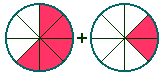
\includegraphics[scale=1]{figuras/fig99.png}
\end{center}
\begin{multicols}{4}
\begin{enumerate}[a)]
	\item $\displaystyle\frac{5}{8}$
	\item $\displaystyle\frac{7}{8}$
	\item $\displaystyle\frac{9}{8}$
	\item $\displaystyle\frac{8}{7}$
\end{enumerate}
\end{multicols}
\end{list}

%==============================================================================================
\subsection{Adição e Subtração de Números Racionais}
\begin{list}{\textbf{Questão \arabic{quest}.}}{\usecounter{quest}}
%define a margem da lista.	
%\setlength{\labelwidth}{-2mm} \setlength{\parsep}{0mm}
%\setlength{\topsep}{0mm} \setlength{\leftmargin}{-2mm}
\renewcommand{\labelenumi}{(\alph{enumi})}

\item Efetue as adições e subtrações.
\begin{multicols}{3}
\begin{enumerate}[a)]
	\item $\displaystyle\left(-\frac{2}{3}\right)+\left(+\frac{1}{4}\right)$
	\item $\displaystyle\left(-\frac{4}{7}\right)+\left(-\frac{2}{6}\right)$
	\item $\displaystyle\left(+\frac{1}{7}\right)-\left(+\frac{1}{3}\right)$
	\item $\displaystyle\left(+\frac{2}{3}\right)-\left(+\frac{1}{3}\right)$
	\item $\displaystyle\left(-\frac{4}{5}\right)-\left(-\frac{1}{8}\right)$
	\item $\displaystyle\left(-\frac{3}{4}\right)- 5$
\end{enumerate}
\end{multicols}

\item Calcule.
\begin{multicols}{2}
\begin{enumerate}[a)]
	\item $(+3,8)+(+5,72)$
	\item $(-1,75)+(+3,84)$
	\item $(+5,5)-(+8,13)$
	\item $(-4,72)-(-0,28)$
\end{enumerate}
\end{multicols}

\item Calcule o valor de cada expressão:
\begin{multicols}{3}
\begin{enumerate}[a)]
	\item $\displaystyle\frac{3}{7}-1+\frac{4}{3}$
	\item $\displaystyle\frac{7}{8}-\frac{1}{4}+\frac{2}{3}$
	\item $-0,25+1,5-0,3$
	\item $-\displaystyle\frac{5}{12}-\frac{1}{12}+\frac{4}{6}$
	\item $0,375-0,125 - 0,625$
	\item $\displaystyle\frac{1}{5}-2+\frac{1}{7}$
\end{enumerate}
\end{multicols}

\item Qual é o valor de cada expressão?
\begin{multicols}{2}
\begin{enumerate}[a)]
	\item $1,7+\left(\displaystyle\frac{2}{3}-0,25\right) - \displaystyle\frac{1}{4}$
	\item $\left[1,6+\left(\displaystyle\frac{1}{4}-0,75+2 \right)-\displaystyle\frac{3}{5}\right]$
\end{enumerate}
\end{multicols}

\item Um submarino encontra-se a $-60$ m de profundidade, se descer o dobro, que profundidade o submarino atingirá?

\item Em certo mês, uma cidade do Sul do país teve sua temperatura máxima de 14,5 ºC e temperatura mínima de $-2,8$ ºC. Qual foi a diferença entre as temperaturas máxima e mínima registradas nesse mês?

\item Lina possuía R\$ 312,50. Recebeu R\$ 250,00 do seu pai e efetuou 3 pagamentos nos valores de R\$ 108,15, R\$ 89,00 e R\$ 204,50. Com quanto Lina ficou?

\item Vitor gastou, em maio, $\frac{1}{3}$ do seu salário com alimentação e $\frac{1}{2}$ com entretenimento, sobrando-lhe ainda R\$ 315,00. Qual foi o salário de Vítor nesse mês?

\item Calcule as somas:
\begin{multicols}{2}
\begin{enumerate}[a)]
	\item $\displaystyle\frac{2}{5}+\left(-\frac{1}{3}\right)$
	\item $\displaystyle\left(-\frac{2}{3}\right)+\left(-\frac{5}{6}\right)$
	\item $\displaystyle\frac{3}{5}+ \left(-\frac{1}{3}\right)+\left(-\frac{2}{5}\right)$
	\item $(+0,1)+(-1,1)+(+0,11)$
\end{enumerate}
\end{multicols}

\item Efetue as subtrações:
\begin{multicols}{2}
\begin{enumerate}[a)]
	\item $\displaystyle\frac{2}{5}-\left(+\frac{1}{4}\right)$
	\item $\displaystyle\left(-\frac{5}{8}\right)-\left(+\frac{3}{8}\right)$
	\item $\displaystyle\left(+\frac{1}{4}\right)-\left(-\frac{1}{2}\right)$
	\item $(-0,54)-(-0,6)$
	\item $-\displaystyle\frac{1}{4}-\left(-\frac{1}{8}\right)$
	\item $\displaystyle\left(-\frac{4}{5}\right)-(+3,8)$
\end{enumerate}
\end{multicols}

\item Calcule o valor das expressões:
\begin{enumerate}[a)]
	\item $\displaystyle\left(+\frac{7}{6}\right)+\left(-\frac{5}{6}\right)$
	\item $\displaystyle\left(+\frac{1}{2}\right)-\left(-\frac{5}{2}\right)+\left(-\frac{3}{2}\right)$
	\item $-\displaystyle\frac{1}{4}+\left(+\frac{3}{5}\right)+\left(-\frac{1}{10}\right)$
	\item $\displaystyle\frac{1}{5}-\left[\frac{2}{3}-\left(\frac{2}{6}-\frac{1}{12}\right)\right]+\frac{5}{6}$
	\item $\left[\left(-\displaystyle\frac{1}{6}\right)+\left(\displaystyle\frac{1}{2}-\frac{1}{3}\right)\right]-\left[\displaystyle\frac{2}{3}+\left(-\frac{1}{2}-\frac{5}{6}\right)\right]$
	\item $[0,4-(0,62-1,8)+(-1,5+1,2)]-0,6$
\end{enumerate}

\item Dê exemplos de dos números racionais cuja soma seja:
\begin{multicols}{4}
\begin{enumerate}[a)]
	\item $-\displaystyle\frac{4}{5}$
	\item $0,7$
	\item $+\displaystyle\frac{1}{2}$
	\item $-6,3$
\end{enumerate}
\end{multicols}

\begin{multicols}{2} 
\item  Determine os números A,B e C da figura, sabendo que a soma dos números situados em qualquer lado é sempre 15.
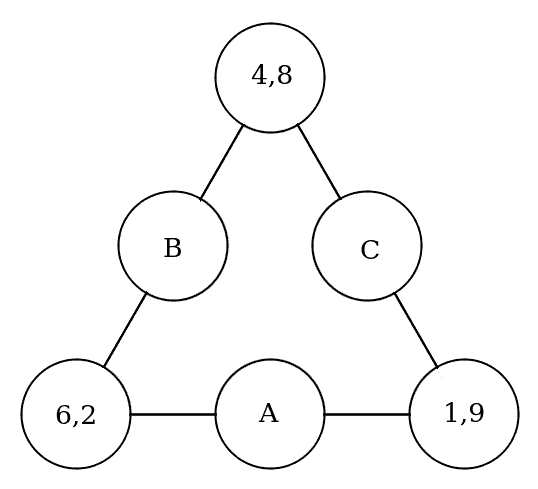
\includegraphics[scale=0.3]{figuras/fig100.png}
\end{multicols}
\end{list}

%==============================================================================================
\subsection{Multiplicação de Números Racionais}
\begin{list}{\textbf{Questão \arabic{quest}.}}{\usecounter{quest}}
%define a margem da lista.	
%\setlength{\labelwidth}{-2mm} \setlength{\parsep}{0mm}
%\setlength{\topsep}{0mm} \setlength{\leftmargin}{-2mm}
\renewcommand{\labelenumi}{(\alph{enumi})}

\item Determine os produtos:
\begin{multicols}{4}
\begin{enumerate}[a)]
	\item $\displaystyle\left(+\frac{2}{3}\right)\cdot\left(-\frac{2}{5}\right)$
	\item $\displaystyle\left(-\frac{3}{4}\right)\cdot\left(-\frac{2}{7}\right)$
	\item $\displaystyle\left(-\frac{3}{5}\right)\cdot\left(+\frac{5}{6}\right)$
	\item $(-0,5)\cdot (-2,0)$
\end{enumerate}
\end{multicols}

\item Determine o valor de cada expressão:
\begin{multicols}{2}
\begin{enumerate}[a)]
	\item $(+2)\cdot \displaystyle\left(-\frac{3}{4}\right)\cdot \left(+\frac{1}{6}\right)$
	\item $\displaystyle\left[\left(-\frac{1}{5}+\frac{3}{4}+1\right)\cdot \left(-\frac{1}{3}\right)\right]$
\end{enumerate}
\end{multicols}

\item Calcule o valor de cada expressão:
\begin{multicols}{2}
\begin{enumerate}[a)]
	\item $(-0,15)\cdot (+0,1)-(+0,6)\cdot (-0,21)$
	\item $(-3)\cdot (-1,6) - (+2)\cdot (-1,3)$
\end{enumerate}
\end{multicols}

\item Calcule o valor das expressões:
\begin{multicols}{3}
\begin{enumerate}[a)]
	\item $(5,4)\cdot (-3,2)$
	\item $(-1,08)\cdot (-2,5)$
	\item $(-3,85)\cdot (+2,4))$
	\item $(+1,4)\cdot (-0,5)$
	\item $(+10,6)\cdot (+8,17)$
	\item $(-8,35)\cdot (-1,17)$
\end{enumerate}
\end{multicols}

\item Efetue as multiplicações.
\begin{multicols}{2}
\begin{enumerate}[a)]
	\item $\left(-\displaystyle\frac{4}{5}\right)\cdot \left(-\displaystyle\frac{7}{4}\right)$
	\item $\left(+\displaystyle\frac{4}{9}\right)\cdot \left(-\displaystyle\frac{16}{81}\right)$
	\item $\displaystyle\left(+\frac{5}{8}\right)\cdot\left(-\frac{4}{3}\right)$
	\item $\left(+\displaystyle\frac{4}{5}\right)\cdot 0$
	\item $(+3)\cdot\displaystyle\left(-\frac{3}{9}\right)\cdot\left(+\frac{18}{6}\right)$
\end{enumerate}
\end{multicols}

\item Isadora vai revestir uma das paredes de seu quarto com um papel decorativo. Essa parede tem 4,35 m de comprimento por 2,80 m de largura. Quantos metros quadrados de papel decorativo serão necessários para cobrir essa parede?

\item Determine o produto dos números $-14$ e $-0,025$.

\item Calcule o valor da expressão: $\left(-\displaystyle\frac{3}{4}\cdot\frac{16}{81} +0,3\right)\cdot \left(-\displaystyle\frac{3}{4}\right)$

\item Em uma sessão de cinema foram vendidos 328 ingressos, sendo 80 meias-entradas. Calcule o valor arrecadado nessa sessão. Sabendo que o preço do ingresso (inteiro) custa R\$ 16,50.

\item Pedro comprou uma moto. Ele pagou $\displaystyle\frac{3}{10}$ de entrada e dividiu o restante em 20 parcelas iguais de R\$ 217,70. Qual foi o valor da moto?
\end{list}

%==============================================================================================
\subsection{Divisão de Números Racionais}
\begin{list}{\textbf{Questão \arabic{quest}.}}{\usecounter{quest}}
%define a margem da lista.	
%\setlength{\labelwidth}{-2mm} \setlength{\parsep}{0mm}
%\setlength{\topsep}{0mm} \setlength{\leftmargin}{-2mm}
\renewcommand{\labelenumi}{(\alph{enumi})}


\item Calcule o valor das divisões.
\begin{multicols}{2}
\begin{enumerate}[a)]
	\item $\left(+\dfrac{1}{4}\right): \left(-\dfrac{1}{2}\right)$
	\item $\left(-\dfrac{2}{5}\right): (+3)$
	\item $\left(-\dfrac{3}{25}\right): \left(-\dfrac{9}{10}\right)$
	\item $(-5):(-10)$
	\item $(-2,5):\left(+\dfrac{2}{100}\right)$
	\item $5:\left(-\dfrac{3}{4}\right)$
\end{enumerate}
\end{multicols}

\item Calcule o valor das expressões.
\begin{enumerate}[a)]
	\item $\left(-\dfrac{3}{4}\right) + \left(-\dfrac{1}{2}\right):\left(+\dfrac{1}{4}\right)$
	\item $\left[(+2) - \left(-\dfrac{3}{2}\right):\left(-\dfrac{3}{2}\right)\right]\cdot\left(-\dfrac{1}{2}\right)$
	\item $\left[\left(+\dfrac{1}{2}\right)\cdot \left(-\dfrac{3}{4}\right) - \left(+\dfrac{1}{2}\right) : \left(-\dfrac{2}{3}\right)\right]: \left(-\dfrac{3}{4}\right)$
	\item $(-3)\cdot (+1,25) - (+1,2) : (0,6)$
\end{enumerate}

\item Determine o valor de:
\begin{multicols}{2}
\begin{enumerate}[a)]
	\item $\dfrac{\left(-\dfrac{2}{5}\right)}{\left(-\dfrac{8}{10}\right)}$
	\item $\dfrac{\left(-\dfrac{1}{2}\right) + \left(+\dfrac{2}{3}\right)}{\left( -\dfrac{1}{6} \right) - \left(-\dfrac{1}{3} \right)}$
	\item $1 + \dfrac{\left(-\dfrac{1}{2}\right)}{\left(-\dfrac{2}{3}\right)}$
	\item $\dfrac{\left(-\dfrac{3}{4}\right)\cdot \left(-\dfrac{2}{5}\right)}{\left(\dfrac{1}{6} \right)}$
\end{enumerate}
\end{multicols}

\item Calcule o valor das expressões.
\begin{multicols}{2}
\begin{enumerate}[a)]
	\item $-27,6:1,5$
	\item $(-4,9):(-0,98)$
\end{enumerate}
\end{multicols}

\item Calcule o valor das expressões.
\begin{multicols}{2}
\begin{enumerate}[a)]
	\item $(-200):(+0,5)$
	\item $(+16,2):(-3,6)$
	\item $(-81,64):(-6,5)$
	\item $(+12,6):(-0,25)$
\end{enumerate}
\end{multicols}

\item Efetue as divisões.
\begin{multicols}{2}
\begin{enumerate}[a)]
	\item $\left(+\displaystyle\frac{7}{6}\right):\left(-\displaystyle\frac{1}{7}\right)$
	\item $\left(-\displaystyle\frac{4}{7}\right):\left(-\displaystyle\frac{8}{7}\right)$
	\item $\left(+\displaystyle\frac{3}{7}\right):\left(+\displaystyle\frac{21}{49}\right)$
	\item $\left(-\displaystyle\frac{3}{5}\right):\left(-\displaystyle\frac{9}{15}\right)$
	\item $\left(-\displaystyle\frac{4}{9}\right):\left(+\displaystyle\frac{16}{81}\right)$
	\item $\left(-\displaystyle\frac{5}{2}\right):(+8)$
	\item $(+16):\left(-\displaystyle\frac{3}{8}\right)$
	\item $\left(-\displaystyle\frac{3}{5}\right):(+0,1)$
\end{enumerate}
\end{multicols}

\item Jorge tinha um terreno de 23 575 metros quadrados. Ele reservou 6 100 metros quadrados desse terreno para área de lazer. Do que restou, Jorge reservou $\displaystyle\frac{1}{5}$ para estacionamento e dividiu o restante em lotes de 349,50 metros quadrados cada um. Quantos lotes Jorge obteve?
\end{list}

%==============================================================================================
\subsection{Potenciação de Números Racionais}
\begin{list}{\textbf{Questão \arabic{quest}.}}{\usecounter{quest}}
%define a margem da lista.	
%\setlength{\labelwidth}{-2mm} \setlength{\parsep}{0mm}
%\setlength{\topsep}{0mm} \setlength{\leftmargin}{-2mm}
\renewcommand{\labelenumi}{(\alph{enumi})}


\item Efetue.
\begin{multicols}{3}
\begin{enumerate}[a)]
	\item $\left(-\dfrac{3}{5}\right)^2$
	\item $\left(+\dfrac{1}{2}\right)^5$
	\item $\left(-1\frac{1}{2}\right)^3$
	\item $(-3,5)^2$
	\item $\left(+\dfrac{1}{3}\right)^0$
	\item $(-1,5)^1$
\end{enumerate}
\end{multicols}

\item Determine o valor de cada expressão.
\begin{enumerate}[a)]
	\item $\left(-\dfrac{1}{2}\right)^2\cdot \left(+\dfrac{3}{2}\right) - \left(+\dfrac{2}{3}\right)^2 : \left(-\dfrac{1}{27}\right)$
	\item $(0,1)^2:(-2) + (1,5)\cdot (-0,1)^2$
\end{enumerate}

\item Calcule as potências.
\begin{multicols}{4}
\begin{enumerate}[a)]
	\item $\left(-\displaystyle\frac{1}{3}\right)^4$
	\item $(0,2)^3$
	\item $(0,01)^2$
	\item $\left(-\displaystyle\frac{17}{20}\right)^0$
	\item $\left(-\displaystyle\frac{1}{2}\right)^4$
	\item $(1,2)^2$
	\item $-0,5^1$
	\item $\left(-\displaystyle\frac{1}{6}\right)^3$
\end{enumerate}
\end{multicols}

\item Calcule o valor das expressões.
\begin{multicols}{2}
\begin{enumerate}[a)]
	\item $\left(-\displaystyle\frac{1}{2}\right)^2 + \displaystyle\frac{3}{4}$
	\item $\left(-\displaystyle\frac{3}{2}\right)^2 + 3\cdot\left(-\displaystyle\frac{1}{2}\right)^3$
\end{enumerate}
\end{multicols}

\item Use a propriedade e escreva diretamente o produto em forma de uma única potência.
\begin{multicols}{2}
\begin{enumerate}[a)]
	\item $10^5\cdot 10^9$
	\item $(-2)^3\cdot (-2)^2$
	\item $\left(\dfrac{1}{2}\right)^2 \cdot \left(\dfrac{1}{2}\right)^3 \cdot \dfrac{1}{2}$
	\item $(1,5)^2 \cdot (1,5)^4$
	\item $ a^2 \cdot a^3 \cdot a^4 \cdot a$ para $a \in \mathbb{Q}$
	\item $\left(-\dfrac{3}{4}\right)^2 \cdot \left(-\dfrac{3}{4}\right)^3 \cdot \left(- \dfrac{3}{4}\right)^4$
\end{enumerate}
\end{multicols}

\item Determine o valor de $x$ e $y$. Considere que $x$ e $y$ são números naturais.
\begin{enumerate}
	\item $2^x \cdot 2^2 \cdot 2^3 = 2^9$
	\item $(-3)^y \cdot (-3)^y \cdot (-3) = (-3)^3$
	\item $2^x \cdot 2^y = 2^6$
	\item $\left(\dfrac{1}{2}\right)^x \cdot \left(\dfrac{1}{2}\right) \cdot \left(\dfrac{1}{2}\right)^x = \left(\dfrac{1}{2}\right)^9$
\end{enumerate}

\item Aplique as propriedades das potências e escreva os resultados por meio de uma só potência.
\begin{multicols}{2}
\begin{enumerate}[a)]
	\item $\left(\displaystyle\frac{7}{13}\right)^{10}:\left(\displaystyle\frac{7}{13}\right)^6$
	\item $\left(-\displaystyle\frac{1}{2}\right)^2\cdot \left(-\displaystyle\frac{1}{2}\right)^4 \cdot \left[ \left( \displaystyle\frac{1}{2}\right)^4 \right]^2$
	\item $\left(\displaystyle\frac{4}{3}\right)^2\cdot\left(\displaystyle\frac{4}{3}\right)^3$
	\item $\left[\left( -0,5\right)^2\right]^3$
	\item $\left[\left( -0,222...\right)^0\right]^{100}$
\end{enumerate}
\end{multicols}
\end{list}

%==============================================================================================
\subsection{Raiz Quadrada de Números Racionais}
\begin{list}{\textbf{Questão \arabic{quest}.}}{\usecounter{quest}}
%define a margem da lista.	
%\setlength{\labelwidth}{-2mm} \setlength{\parsep}{0mm}
%\setlength{\topsep}{0mm} \setlength{\leftmargin}{-2mm}
\renewcommand{\labelenumi}{(\alph{enumi})}


\item Efetue.
\begin{multicols}{3}
\begin{enumerate}[a)]
	\item $\sqrt{\dfrac{36}{64}}$
	\item $\sqrt{+0,04}$
	\item $\sqrt{+0,25}$
	\item $\sqrt{-\dfrac{1}{9}}$
	\item $\sqrt{+1\frac{7}{9}}$
	\item $\sqrt{3,24}$
\end{enumerate}
\end{multicols}

\item Determine o valor de cada expressão.
\begin{multicols}{2}
\begin{enumerate}[a)]
	\item $\dfrac{1}{2}\cdot \sqrt{1,69} + \dfrac{2}{5}\cdot \sqrt{0,81}$
	\item $2\cdot \sqrt{0,36} - 5\cdot \sqrt{0,09} + (-3)$
\end{enumerate}
\end{multicols}

\item Calcule, se possível, as raízes quadradas.
\begin{multicols}{4}
\begin{enumerate}[a)]
	\item $\sqrt{\displaystyle\frac{100}{9}}$
	\item $-\sqrt{\displaystyle\frac{1}{81}}$
	\item $-\sqrt{0,01}$
	\item $\sqrt{\displaystyle\frac{4}{25}}$
	\item $\sqrt{6,25}$
	\item $\sqrt{\displaystyle\frac{-81}{64}}$
	\item $-\sqrt{\displaystyle\frac{1}{144}}$
	\item $\sqrt{0,64}$
\end{enumerate}
\end{multicols}

\item calcule o valor de cada uma das expressões.
\begin{multicols}{2}
\begin{enumerate}[a)]
	\item $\dfrac{2}{\sqrt{81}}-\dfrac{\sqrt{16}}{3}+\dfrac{2}{\sqrt{25}}-\dfrac{\sqrt{36}}{3}$
	\item $ \sqrt{\dfrac{4}{25}}-\sqrt{\dfrac{1}{9}}+\sqrt{\dfrac{9}{25}}-\sqrt{\dfrac{4}{9}}$
	\item $\sqrt{\dfrac{1}{25}}\cdot\sqrt{\dfrac{25}{9}}\cdot\left(\sqrt{\dfrac{9}{4}}\right)^2 - \sqrt{\dfrac{1}{16}}$	
\end{enumerate}
\end{multicols}
\end{list}

%==============================================================================================
\subsection{Expressões Numéricas com Números Racionais}
\begin{list}{\textbf{Questão \arabic{quest}.}}{\usecounter{quest}}
%define a margem da lista.	
%\setlength{\labelwidth}{-2mm} \setlength{\parsep}{0mm}
%\setlength{\topsep}{0mm} \setlength{\leftmargin}{-2mm}
\renewcommand{\labelenumi}{(\alph{enumi})}

\item Calcule o valor numérico de cada expressão.
\begin{multicols}{2}
\begin{enumerate}[a)]
	\item $\left(-2 - \dfrac{2}{5}\right)\cdot \left(-\dfrac{3}{4}\right)^2$
	\item $1-\left(\dfrac{1}{3}\right)^2:\left(\dfrac{1}{2}-1\right)^2$
	\item $\left(0,1+\dfrac{1}{5}\right):\left(-0,02+\dfrac{1}{100}\right)$
	\item $\left(\dfrac{1}{5} - \dfrac{1}{2}\right) - \left(\dfrac{1}{3} - \dfrac{1}{4}\right)\cdot \dfrac{2}{5}$
	\item $-\dfrac{5}{8} + \dfrac{1}{4}\cdot(0,2) + \dfrac{1}{2} $
\end{enumerate}
\end{multicols}

\item Resolva as expressões numéricas.
\begin{enumerate}
	\item $\left(\dfrac{\dfrac{7}{5}}{\dfrac{14}{4}} - 0,15\right) : (1 -3 \cdot 0,4)$
	\item $\left(\dfrac{1}{3}\right)^2 - \sqrt{\dfrac{1}{16}}\cdot \left[\dfrac{3}{4} - \left(-2 + \dfrac{3}{2}\right)^2\right]$
\end{enumerate}

\item Calcule o valor das expressões.
\begin{multicols}{2}
\begin{enumerate}[a)]
	\item $\dfrac{3 - \dfrac{1}{4}}{1 + \dfrac{2}{5}}$
	\item $\dfrac{-10}{2 - \dfrac{3}{2}}$
\end{enumerate}
\end{multicols}

\item Calcule o valor numérico das expressões.
\begin{enumerate}
	\item $2x-9y$, sendo: $x = -\dfrac{1}{4}$ e $y = \dfrac{1}{3}$
	\item $x^2 + 2xy$, sendo: $x = -\dfrac{1}{3}$ e $y = \dfrac{1}{4}$
	\item $2x^2 - 4y + 8$, sendo: $x = 2^{-2}$ e $y = 2^{-3}$
\end{enumerate}

\item Calcule o valor das expressões.
\begin{enumerate}[a)]
	\item $[(-7)^6\cdot (-7)^8\cdot (-49)^3]^2:(-7)^{18}$
	\item $[(-0,03)^7\cdot (-0,03)^3\cdot(0,03)]:(-0,03)^8$
\end{enumerate}
\end{list}

%==============================================================================================
\subsection{Potências com expoentes inteiros.}
\begin{list}{\textbf{Questão \arabic{quest}.}}{\usecounter{quest}}
%define a margem da lista.	
%\setlength{\labelwidth}{-2mm} \setlength{\parsep}{0mm}
%\setlength{\topsep}{0mm} \setlength{\leftmargin}{-2mm}
\renewcommand{\labelenumi}{(\alph{enumi})}

\item Calcule as potências. Nas potências de expoente negativo, dê a resposta na forma decimal.
\begin{multicols}{4}
\begin{enumerate}[a)]
	\item $10^6$
	\item $10^{-6}$
	\item $10^{-4}$
	\item $10^4$
	\item $10^{-2}$
	\item $10^{-5}$
	\item $10^{10}$
	\item $10^{-8}$
\end{enumerate}
\end{multicols}

\item Escreva os números seguinte como potências de base 10.
\begin{multicols}{4}
\begin{enumerate}[a)]
	\item 1000
	\item 0,001
	\item $\displaystyle\frac{1}{10\ 000}$
	\item 10 000 000
	\item 0,00001
	\item 100 000 000 000
	\item 1
	\item $1000\cdot10\ 000$
\end{enumerate}
\end{multicols}

\item Escreva a decomposição dos seguintes decimais usando potências de 10.
\begin{multicols}{4}
\begin{enumerate}[a)]
	\item 3,49
	\item 31,6
	\item 17,043
	\item 109,306
\end{enumerate}
\end{multicols}

\item Simplifique cada uma destas expressões escrevendo-as como uma única potência de 10.
\begin{multicols}{2}
\begin{enumerate}[a)]
	\item $\displaystyle\frac{10^5\cdot 10^{-3}\cdot 10^2}{10^{-4}\cdot 10^7}$
	\item $\displaystyle\frac{10^4\cdot 10^{-6}\cdot 10^2}{10^{3}\cdot 10\cdot 10^{-3}}$
\end{enumerate}
\end{multicols}

\item Escreva os números a seguir em notação científica.
\begin{multicols}{3}
\begin{enumerate}[a)]
	\item 49 000 000 000
	\item 0,00000607
	\item 9 360 000
	\item 0,00001
	\item 10 000 000 000 000
	\item 0,00007
\end{enumerate}
\end{multicols}
\end{list}
%==============================================================================================
\subsection{Grandezas e suas Unidades}
\subsubsection{Tabela de Grandezas}
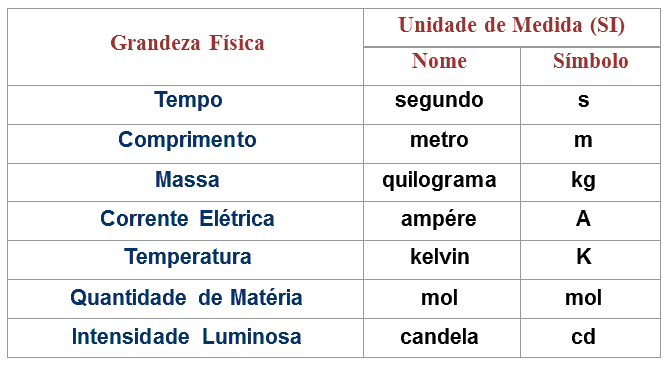
\includegraphics[scale=1]{figuras/tabela_grandeza_unidade.png}
\subsubsection{Conversão de Valores}
\begin{multicols}{2}
\begin{flushleft}
Comprimento.
\end{flushleft}
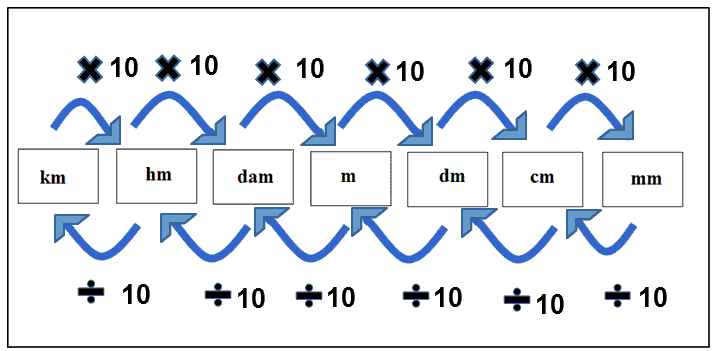
\includegraphics[scale=0.3]{figuras/conversao_comprimento.png}
\begin{flushleft}
Área.
\end{flushleft}
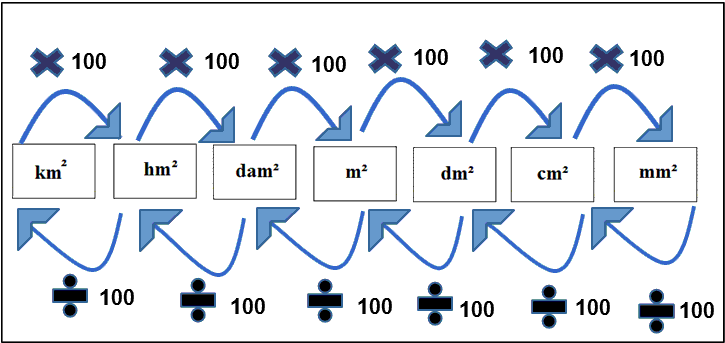
\includegraphics[scale=0.3]{figuras/conversao_area.png}
\begin{flushleft}
Massa.
\end{flushleft}
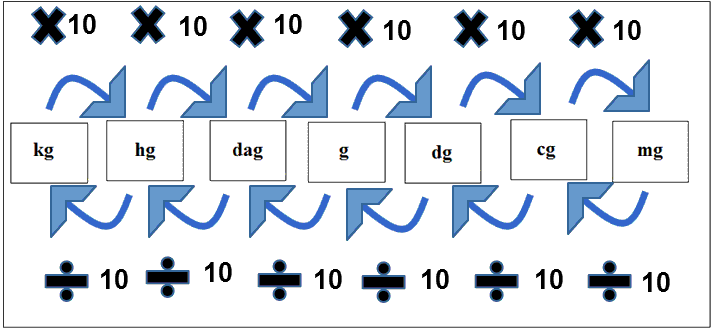
\includegraphics[scale=0.3]{figuras/conversao_massa.png}
\begin{flushleft}
Tempo.
\end{flushleft}
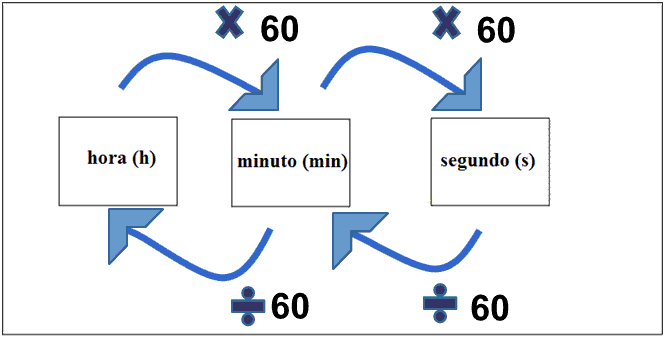
\includegraphics[scale=0.3]{figuras/conversao_tempo.png}
\end{multicols}


